\chapter{基于多传感器的无人机引导系统设计}
\section{引言}
在引导无人机降落过程中,可见光传感器容易受到环境光变化和舰船运动的扰动,进而影响对无人机相对位置的解算。此外,当无人机出现在距离期望降落点较远的距离时,立体视觉在深度方向的解算精度相对较差。考虑到可见光引导系统的上述缺陷,本章主要通过引入激光反射器、红外相机和超宽带雷达等传感器,提高对无人机目标的深度探测精度并降低无人机目标识别和跟踪难度,通过分析舰船运动和着舰点运动特点,对无人机的降落决策进行分析和设计。

\section{多传感器引导架构}
\subsection{激光主动成像技术}
为增强在无人机距离较远时($1\ km$以上)的识别率和跟踪准确性,本文提出一种使用激光照射器和反射器来实现的方法。在激光主动成像技术中,激光波长的选择影响目标的成像质量。在无人机降落过程中的海空背景,除太阳外,一般较少出现主动发光的光源。通过分析红外大气窗口等信息可知,$940\ nm$波段处于红外光吸收带。

本文选用选用山东神戎电子股份有限公司生产的SHR-JLI1000激光照明器,该设备主要产生$940\ nm$波段的激光,其发射功率为$25\ w$。在无人机前端,通过安装全反射棱镜来使得接收到的激光按原光路返回。此外,通过在可见光镜头前添加$940\ nm$的窄带滤光片来实现其他波段光源的干扰。激光主动成像技术设备的安装方案如图\ref{fig:chp06_07_laser}所示。

\begin{figure}[!h]
	\centering
	\includegraphics[width=\textwidth]{figs/chp06/chp06_07_laser.pdf}	
	\caption{激光照射器、全反射棱镜和UWB定向天线}
	\label{fig:chp06_07_laser}
\end{figure}

在可见光相机在添加窄带滤光片后,成像激光点相对简单,背景噪声相对较小,本文采用简单的Hough圆提取方式即可实现对目标的跟踪和识别,其基本识别流程图如图\ref{fig:chp06_02_laser_point_detect}所示。

\begin{figure}[!t]
	\centering
	\includegraphics[width=1.0\textwidth]{figs/chp06/chp06_02_laser_point_detect.pdf}	
	\caption{激光照射点的目标识别与跟踪方法}
	\label{fig:chp06_02_laser_point_detect}
\end{figure}

Hough变换(Hough Transform)是由Hough Paul于1962年在一份专利报告中提出\cite{vc1962method}
由保罗·霍夫在1962年提出的Hough变换是一种比较经典的检测不同形状的方法,在由激光主动成像与全反射棱镜配合得到的图像中,目标是以圆形亮斑呈现的,因此本文在对图像进行Canny边缘提取之后,使用Hough变换从中提取出目标所呈现的圆形。在无人机降落过程中,位于$1000\ m$和$1500\ m$处的成像结果如图\ref{fig:chp06_10_1000_1500_Hough}所示。

\begin{figure}[!t]
	\centering
	\includegraphics[width=1.0\textwidth]{figs/chp06/chp06_10_1000_1500_Hough.pdf}	
	\caption{激光照射点成像结果}
	\label{fig:chp06_10_1000_1500_Hough}
\end{figure}


\subsection{红外成像技术}
红外热像仪是利用红外探测器和光学成像物镜接受被测目标的红外辐射能量,将分布图形反映到红外探测器的光敏元件上,从而获得红外热像图,这种热像图与物体表面的热场分布相对应。本系统选用的浙江大力科技股份有限公司生产的红外热像仪CM6240FC,大气能见度大于$10\ km$,相对湿度小于$80\%$,目标与背景温差3K条件下,对$3\ m\times3\ m$的目标,探测距离不小于$7\ km$,识别距离不小于$5\ km$。$对1.7\ m\times0.5\ m$目标(人),探测距离不小于$5\ km$,识别距离不小于$2.5\ km$。本文实验中使用的四旋翼目标和固定翼目标的成像结果如图\ref{fig:chp06_11_uav_landing}所示。

\begin{figure}[!t]
	\centering
	\includegraphics[width=1.0\textwidth]{figs/chp06/chp06_11_uav_landing.pdf}	
	\caption{红外目标成像结果}
	\label{fig:chp06_11_uav_landing}
\end{figure}

\subsection{超宽带雷达}
超宽带无线测距以其高距离的分辨力、强穿透力、低截获率以及很强的抗干扰能力在军事、商业等领域得到越来越多的关注。本文使用的UWB型号为Time Domain公司的PulsONP410。P410的RF传输频率$3.1\ GHz$到$5.3\ GHz$,中心频率位于$4.3\ GHz$附近。该设备探测距离$2\ km$以上,如果选用增强型的定向天线探测距离可以达到$5\ km$以上。该设备安装在二自由度转台和无人机机头位置,如图\ref{fig:chp06_07_laser}所示。

加入定向天线后,UWB的探测波半角为$20\degree$,当远距离无人机进入探测窗口时,UWB可以探测到目标。当无人机距离目标$500\ m$、水平位置为$10\ m$,高度为$30\ m$时,UWB的精度为$0.5\ m$。水平方向的误差为$0.01\ m$,高度为$0.03\ m$,该精度低于可见光解算的无人机深度距离的系统误差。

\section{基于EKF的转台信息滤波解算}
\subsection{位置和姿态估计方法分析}
位姿估计问题(Pose Estimation)是估计特定物体相对于参考坐标系的位置和姿态。在传统方法中,GPS、惯性测量单元(IMU)、视觉、激光雷达等作为主要传感器来对目标进行估计和判断。位姿估计问题既可以只依赖视觉传感器,也可以综合应用各类型传感器采集到的数据通过滤波得到。在以视觉信息为主的位姿估计方法中,主要有一下两类方法:(1)单目视觉。单视觉方法主要依赖对平面的检测、合作标志的检测、海天线或地平面的检测。(2)多目视觉。多目视觉方法主要指针对特征点在不同成像平面的位置,通过多个相机的排布,从而解算出目标的位置和姿态信息。

\subsection{EKF方法状态模型设计}
基于视觉的位姿估计问题主要应用于人机交互(Human Computer Interaction)、视觉里程计(VO)和机器人导航和实时定位与建图(SLAM)。其中,视觉里程计主要通过对系列连续图像进行处理,结合飞行器自身携带的各类传感器,最终得到可靠的三维信息(3D motion)。针对长基线系统,利用EKF方法,将转台信息和图像信息相融合,可以得到较好的目标位置状态。定义$X$是状态模型
\begin{equation}
X=[Pos^s, V^s, C^{Att}, w^{Att}]^T
\end{equation}
其中
$$
Pos^s=\left[\begin{array}{c}
x_l\\
y_l\\
z_l\\
\end{array}\right],
V^s=\left[\begin{array}{c}
v_x\\
v_y\\
v_z\\
\end{array}\right]
$$
$$
C^{Att}=\left[\begin{array}{c}
lpan\\
ltilt\\
rpan\\
rtilt\\
\end{array}\right],
w^{Att}=\left[\begin{array}{c}
wlpan\\
wltilt\\
wrpan\\
wrtilt\\
\end{array}\right].
$$
上述所有变量均定义在引导系统坐标系。其中$lpan$ 和 $ltilt$ 表示左侧相机的俯仰角度和水平角度; $rpan$ 和 $rtilt$ 对应右侧相机的两个角度; $wlpan, wltilt, wrpan, wrtilt$ 表示上述四个角度的角速度。
在第$k$次迭代过程中,状态转换方程如下
\begin{equation}
\bar{x}_{k|k_1}=F_k\bar{x}_{k-1|k-1}
\end{equation}
其中$F_k$是状态转换矩阵。根据EKF的基本假设,在第$k$时刻的状态只从第$k-1$时刻得到。因此可以得到目标的预测位置和相机的姿态解算公式,
\begin{equation}
\overline{Pos}^s_{k|k-1}=\Delta t V^s_{k-1|k-1} + {Pos}^s_{k-1|k-1}
\end{equation}
\begin{equation}
\overline{C}^{Att}_{k|k-1}=\Delta t w^{Att}_{k-1|k-1} + \overline{C}^{Att}s_{k-1|k-1}
\end{equation}
其中$\Delta t$表示相邻两次时间间隔。状态转换方程可以写为,
\begin{equation}
\bar{x}_{k|k-1}=\left[\begin{matrix}
I_{3\times 3} & \Delta t_{3\times 3} & \textbf{0}_{3\times 4} & \textbf{0}_{3\times 4}\\
\textbf{0}_{3\times 3} & I_{3\times 3} & \textbf{0}_{3\times 4} & \textbf{0}_{3\times 4}\\
\textbf{0}_{4\times 3} & \textbf{0}_{4\times 3} & I_{4\times 4} & \Delta t_{4\times 4}\\
\textbf{0}_{4\times 3} & \textbf{0}_{4\times 3} & \textbf{0}_{4\times 4} & I_{4\times 4}\\
\end{matrix}\right]\bar{x}_{k-1|k-1}
\end{equation}
其中$\Delta t_{n \times n}$表示$n \times n$阶矩阵,其对角线位置为$\Delta t$,其余位置为0。在第$k$时刻,系统的协方差矩阵为,
\begin{equation}
P_{k|k-1}=F_kP_{k-1|k-1}F^T_k+G_kQ_kG^T_k
\end{equation}
其中$Q_k$是动态系统的高斯噪声,$G_k$是第$k$时刻$Q_k$的Jacobian矩阵。状态协方差矩阵由四个部分组成,分别对应:目标-目标、目标-相机、相机-相机和相机-目标,其公式为
\begin{equation}
P_k=\left[
\begin{matrix}
P_{T|T} & P_{T|C} \\
P_{C|T} & P_{C|C} \\
\end{matrix}\right].
\end{equation}
\subsection{EKF方法观测模型设计}
EKF的观测模型基于传统的相机成像模型和映射模型,测量向量$z$为,
\begin{equation}
z=[Pos^I_L, Pos^I_R, C^{PTU}]^T
\end{equation} 
其中$Pos^I_L$和$Pos^I_R$分别表示目标在左右相机的位置,$(u^L_k, v^L_k)$和$(u^R_k, v^R_k)$表示目标在相平面的位置。此时,假设相机光心位置和PTU转台位置在运动过程中保持不变,即忽略安装偏移误差。为了计算目标在相平面的位置,将相机位置、内参数等引入方程
\begin{equation}
\left[\begin{matrix}
\overline{Pos}^I \\
1\\
\end{matrix}\right]
=h(\overline{Pos}^s_{k|k-1}, \overline{C}^{Att}_{k|k-1})
=\lambda N^{in}\overline{M}^{out}_{k|k-1}\overline{Pos}^s_{k|k-1}
\end{equation}
其中$\lambda$是归一化参数。$N^{in}$和$\overline{M}^{out}_{k|k-1}$是转换矩阵。其他参数可以通过如下方程表达,
\begin{equation}
\overline{M}^{out}_{k|k-1}
= \left[
\begin{matrix}
\bar{R}^c_{k|k-1} & T \\
\textbf{0}^T_3 & 1 \\
\end{matrix}
\right]
\end{equation}
和
\begin{equation}
N^{in}=
\left[
\begin{matrix}
1/d_x & 0 & u_o \\
0 & 1/d_y & v_0 \\
0 & 0 & 1 \\
\end{matrix}
\right]
\left[
\begin{matrix}
f & 0 & 0 & 0 \\
0 & f & 0 & 0 \\
0 & 0 & 0 & 1 \\
\end{matrix}
\right]
\end{equation}
其中$\bar{R}^c_{k|k-1}$是旋转矩阵$\overline{C}^{Att}_{k|k-1}$和$T$描述相机坐标系和引导系统坐标系之间的位置关系。由此,可以推导出观测模型为
\begin{equation}
\bar{z_k}=
\left[
\begin{matrix}
\overline{Pos}^I_L \\
\overline{Pos}^I_R \\
\overline{C}^{PTU} \\
\end{matrix}
\right]
=
\left[
\begin{matrix}
Block (\lambda_L N^{in}_L \overline{M}^{out}_{L(k|k-1)}\overline{Pos}^s_{k|k-1} )\\
Block (\lambda_R N^{in}_R\overline{M}^{out}_{R(k|k-1)}\overline{Pos}^s_{k|k-1}  )\\
I_{4 \times 4}\overline{C}^{Att}_{k|k-1} \\
\end{matrix}
\right]
\end{equation}
定义$Block(\cdot)$作为仅提取矩阵前两项的函数。

$x_k$是$z_k$的更新结果。根据观测模型$h$,其Jacobian矩阵$H_k$可以表达为
\begin{equation}
H_k=\frac{\partial h ( \overline{Pos}^S_{k|k-1}, \overline{C}^{Att}_{k|k-1} )}{\partial x_k} 
\end{equation}
得到卡尔曼增益$K_t$,
\begin{equation}
S_k=H_k P_{k|k-1} H^T_k + R
\end{equation}
\begin{equation}
K_k=P_{k|k-1}H^T_k(S_k)^{-1}
\end{equation}
其中$R$是传感器的高斯白噪声。最后,得到更新方程,
\begin{equation}
\bar{x}_{k|k} = \bar{x}_{k|k-1}+K_k(z_k-h(\bar{x}_{k|k-1}))
\end{equation}
\begin{equation}
P_{k|k}=(1-K_k H_k)P_{k|k-1}
\end{equation}
目标识别方法的输出做为EKF的输入,随后将EKF输出结果通过数据链路返回给无人机。

\section{舰船运动估计模型}
\subsection{海浪模型设计}
由于舰载引导系统与船体固连,在浪涌的影响下,引导系统会随舰体同时运动,因此无人机下降过程中需要考虑这类扰动对期望期望着舰点带来的影响。一般而言,海风是直接引起风浪的直接原因,但海风停止后,影响仍然存在。浪涌对船体的影响具有一定的周期性,本文主要通过采集和仿真环境和真实舰船或附体的运动数据,通过安装与舰体固连IMU传感器的方法,将传感器提供的六个自由度的数据进行处理和分析,对当前舰船的姿态进行解算,并对未来一定周期的期望舰船期望姿态进行估计。美国海军规定着舰时船体姿态运动的范围:纵摇不得超过$2\degree$,横摇不得超过$7\degree$,升沉幅度不得超过$3\ m$,升沉率不得超过±$3\ m/s$,而舰尾的下沉量不得超过$1.5\ m$。

根据国家海洋局公布的名词解释,海况的基本等级通常用道氏波级(Douglas Sea Scale)进行描述\cite{sea_state}。这种描述方法的通过定义海浪的显著高度来对海况进行了分类,但在一定程度上忽略了水波的周期性特性,无法直接用于对舰船运动特点进行建模和分析。为进一步描述海况,Haver和Moan在1985年发表的文章\cite{haver1983some}中指出海浪的起伏状态是一个随机过程,在长周期情况下,海浪的时域和空域状态难以准确预测,但在短周期存在一定规律。该文章的作者在大西洋上设置浮标,收集和分析4586组海浪数据后得到短周期海浪模型:(1)在低等海况条件下(最大海浪高度小于4米)时,海浪的运动周期约为20分钟,运动状态符合高斯假设。(2)在中等海况情况下(最大海浪高度小于8米),高斯模型开始出现偏差,但仍在一定情况下描述海况。因此,海浪的波形可以视为由多个频率、相位和振幅不同的正弦函数叠加而成。因为正弦波独有的频域特性,对海浪的分析和描述主要采用傅里叶变换和谱分析方法。

皮尔逊-莫斯科维奇(Pierson-Moskowitz)海浪谱方法于1961年被提出,该方法描述了海浪的能量分布情况,是一种充分发展海普(Fully Developed Sea Spectrum),其公式如下:
\begin{equation}
 S_{PM}(\omega) =\frac{0.78}{\omega^5}\exp(\frac{-3.11}{\omega^4h^2})\ \ (m^2sec)
\end{equation}
 其中普频率的峰值为$\omega_0=1.26\sqrt{h}$,$h$为显著浪高(Significant Wave)。为了更准确的描述海况,该公式在1978年被进一步修正为
\begin{equation}
\mathbf{S}_{\zeta \zeta}(\omega) = \frac{A}{\omega^5}\exp(\frac{-B}{\omega^4})
\end{equation}
其中$A=\frac{487h^2}{T_0^4}$,$B=\frac{1949}{T_0^4}$,$T_0=\frac{2\pi}{\omega_{peak}}$,$\omega_{peak}$定义为主波频率。

因为海浪在风向不同的影响会产生不同影响,所以上式需要在传播方向和传播尺度上进行进一步描述,由此得到
\begin{equation}
\mathbf{S}_{\zeta\zeta,s}(\omega,\chi) = \mathbf{S}_{\zeta\zeta}(\omega)M(\chi,s)
\end{equation}
其中$\chi$描述海浪的传播方向,$s$描述海浪传播尺度因子。

无人机在着舰过程中,一般会选择相对较好的气候条件进行(不高于四级海况),因此皮尔逊-莫斯科维奇海浪谱方法能够满足我们对海况分析的需求。关于该方法更详细的描述和其他方法的讨论可以参阅文献\cite{perez2002simple}。
 
图\ref{fig:wave_spectrum_30}主要描述了在设定风向为$\chi =30\degree$,显著浪高为$h  =2.5\ m$(即四级海况),波浪传播等级参数$s=2$时的波谱图,基于该波谱图。可以随机产生$500\ m \times 500\ m$范围的海浪模型,如图\ref{fig:sea_state_realization_zip}所示。右侧色带描述了不同位置海浪的高度。
 \begin{figure}[!ht]
 	\centering
 	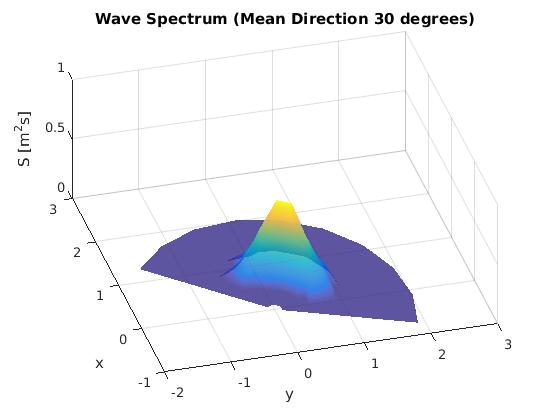
\includegraphics[width=0.7\textwidth]{figs/chp06/wave_spectrum_30.pdf}	
 	\caption{风向为$30\degree$,浪高为$2.5\ m$时的海况情况}
 	\label{fig:wave_spectrum_30}
 \end{figure}

 \begin{figure}[!ht]
	\centering
	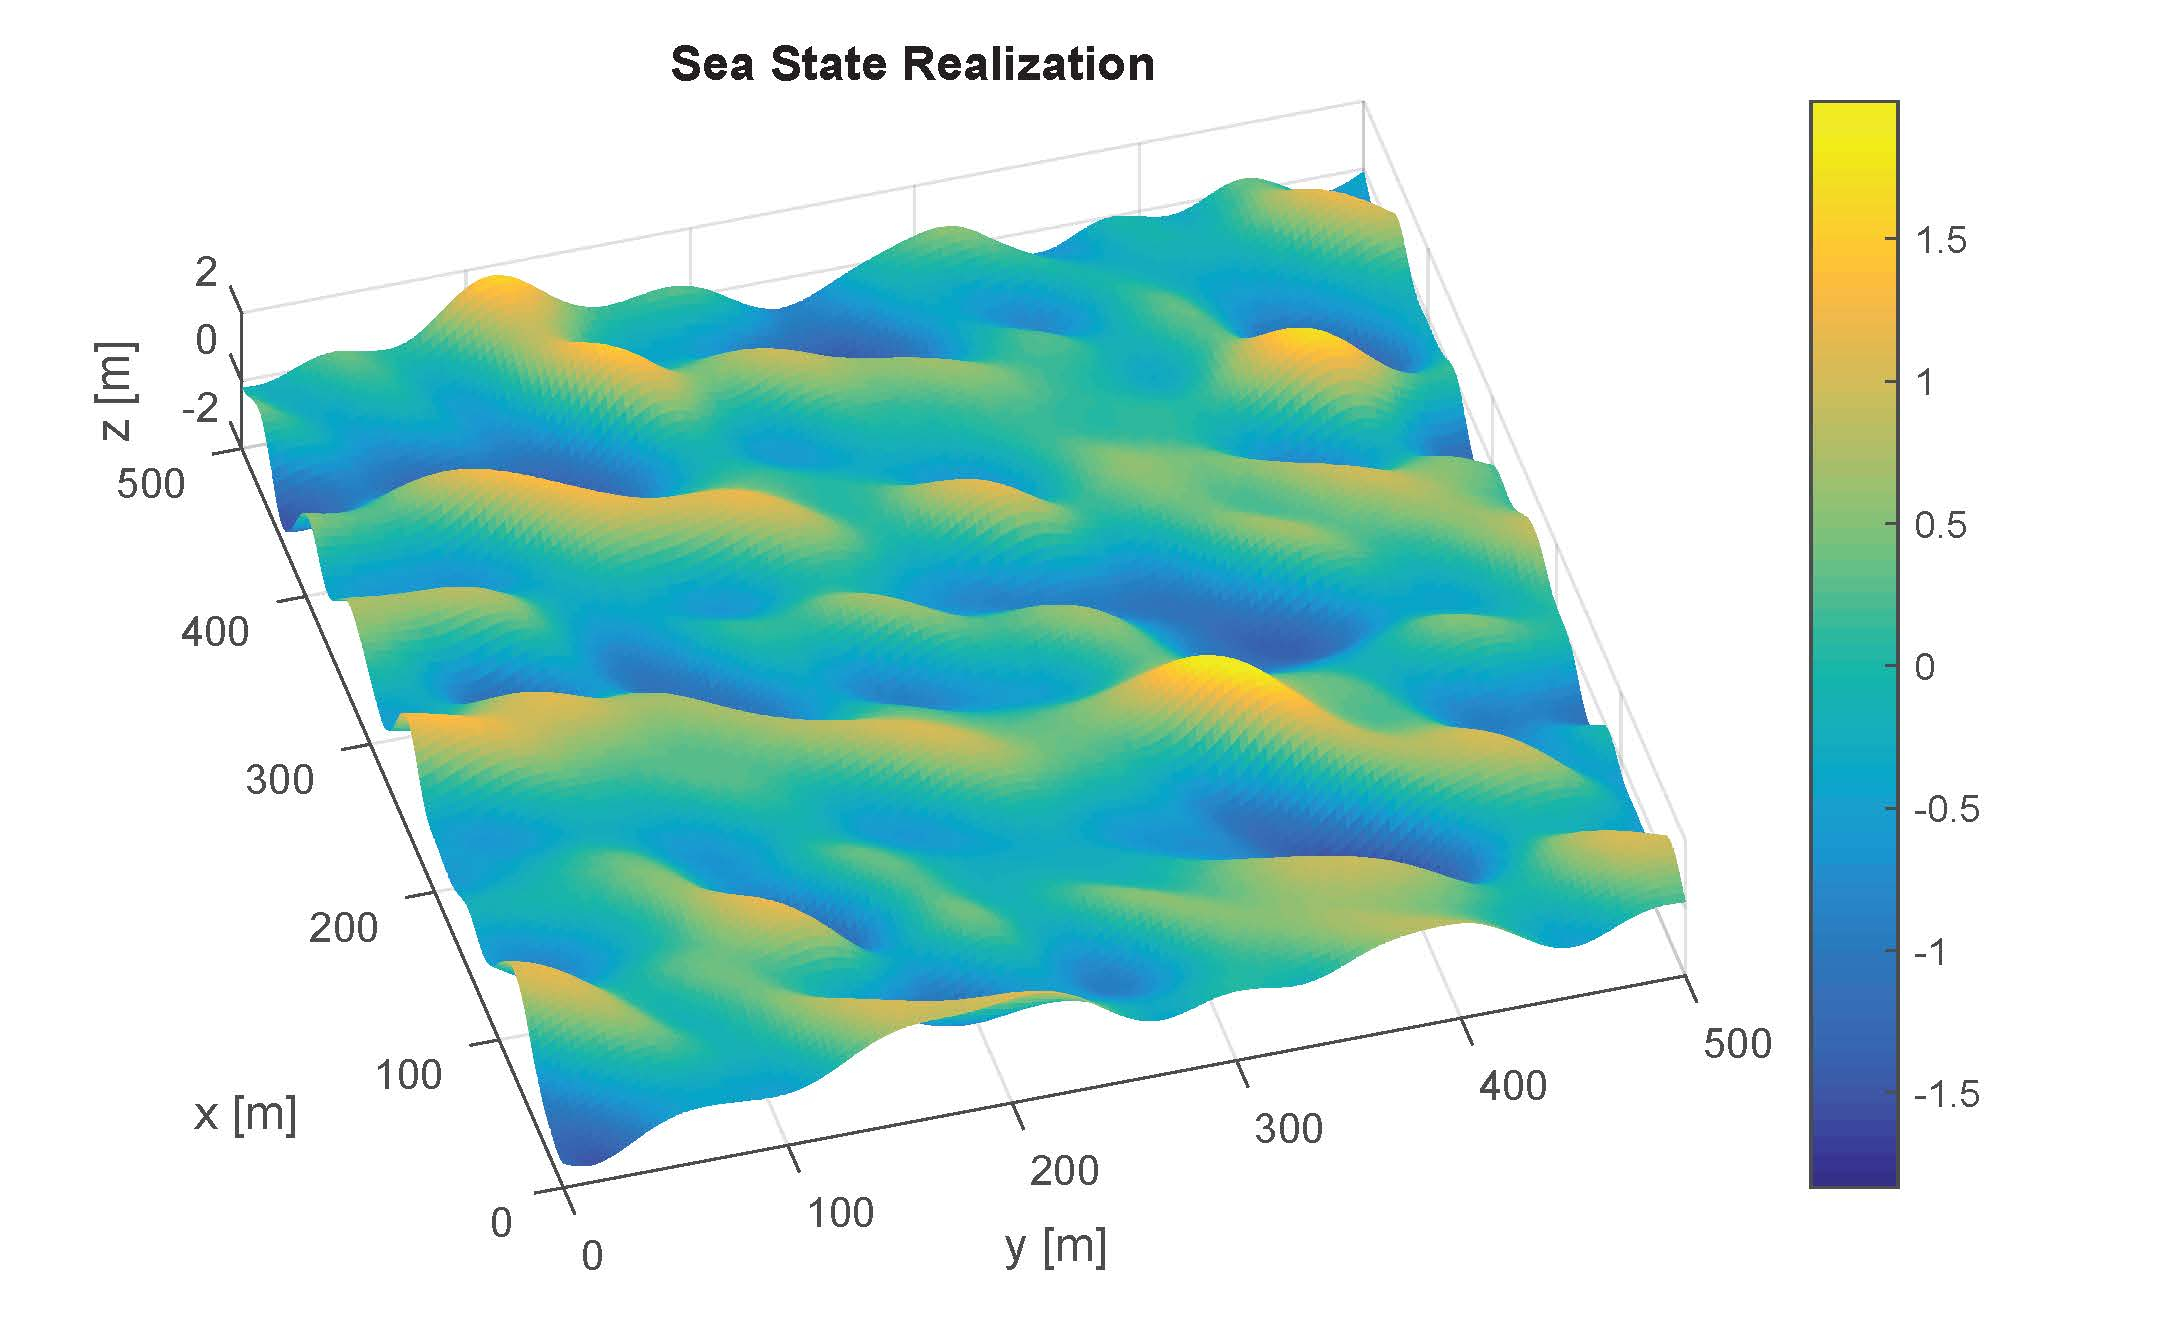
\includegraphics[width=0.7\textwidth]{figs/chp06/sea_state_realization_zip.pdf}	
	\caption{海浪模型}
	\label{fig:sea_state_realization_zip}
\end{figure}

\subsection{舰船运动分析}
在海况模型建立之后,需要对船体的模型进行设计,结合海况模型和船体模型可以得到期望着舰点的运动模型并估计其短周期运动位置。在船舶和浮体设计领域,一般通过定义舰船摇荡响应幅值算子(Response Amplitude Operators,RAO)来描述舰船在不同海况下的运动行为,该算子主要通过流体力学仿真(CFD)软件计算或通过缩比模型的水池实测得到。其基本框图为

 \begin{figure}[!ht]
	\centering
	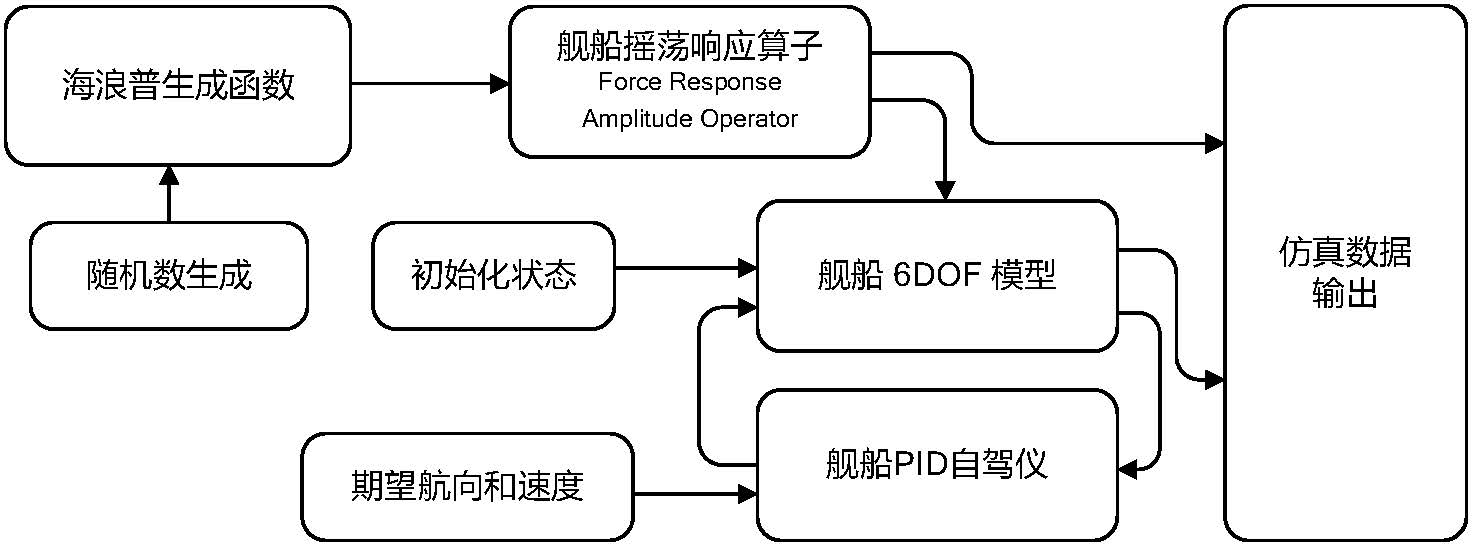
\includegraphics[width=\textwidth]{figs/chp06/01_Visio_wave_sys.pdf}	
	\caption{海浪对舰船影响分析框图}
	\label{fig:01_Visio_wave_sys}
\end{figure}
根据文献\cite{fitzgerald2004flight}中的数据,在舰载机降落和起飞时,航母的运行时速一般在20节至30节(约65公里/小时)之间。根据上一节海浪产生的模型,对舰船在逆风航行($\psi=225\degree$)和侧风航行($\psi = 180\degree\  or\  270\degree$)时,舰船时速为$10\ m/s$(约20节)情况的运动轨迹,如图\ref{fig:wave_30_height_25_comparision_pos}所示。(这里不采用210°,即完全逆风航行的原因是,考虑到真实情况下风向存在一定的变化,因此舰船航向角无法完全逆风行驶。)
 \begin{figure}[!ht]
	\centering
	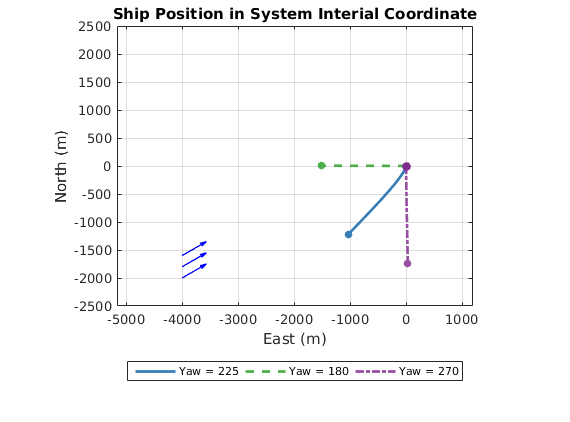
\includegraphics[width=0.7\textwidth]{figs/chp06/wave_30_height_25_comparision_pos.pdf}	
	\caption{风向为$30\degree$,浪高为$2.5\ m$时的海况情况}
	\label{fig:wave_30_height_25_comparision_pos}
\end{figure}
图中的坐标系为系统坐标系,蓝色三个箭头表示海风的方向,三个不同颜色的轨迹描述舰船在期望横向角不变的情况下,180秒的的运动轨迹。由于受到风浪的影响,舰船的轨迹出现一定的偏差。舰船在这三种不同航向情况下,六个自由度的状态如图\ref{fig:wave_30_height_25_comparision_xyz}和图\ref{fig:wave_30_height_25_comparision_rpy}所示。

 \begin{figure}[!ht]
	\centering
	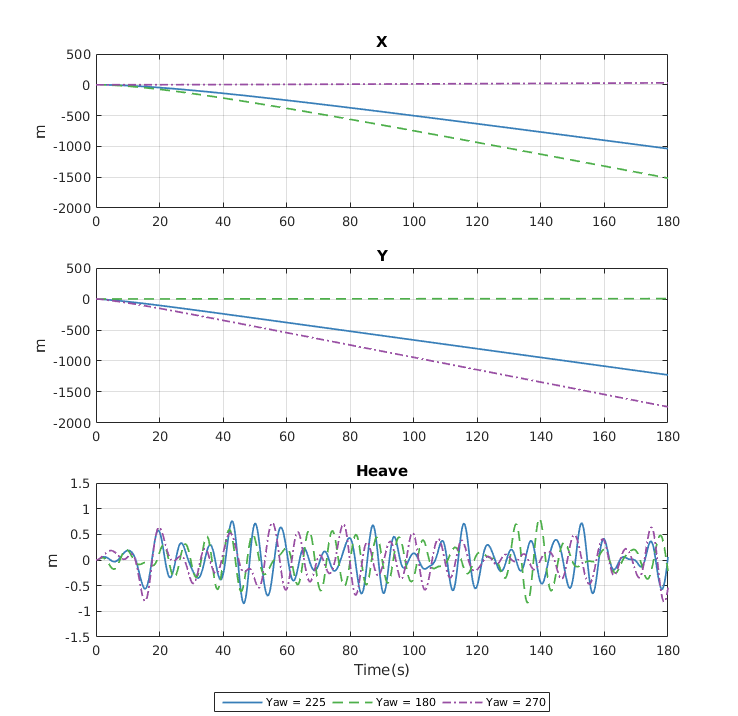
\includegraphics[width=0.7\textwidth]{figs/chp06/wave_30_height_25_comparision_xyz.pdf}	
	\caption{风向为$30\degree$,显著浪高为$2.5\ m$的海况下,三个坐标轴的情况}
	\label{fig:wave_30_height_25_comparision_xyz}
\end{figure}
 \begin{figure}[!ht]
	\centering
	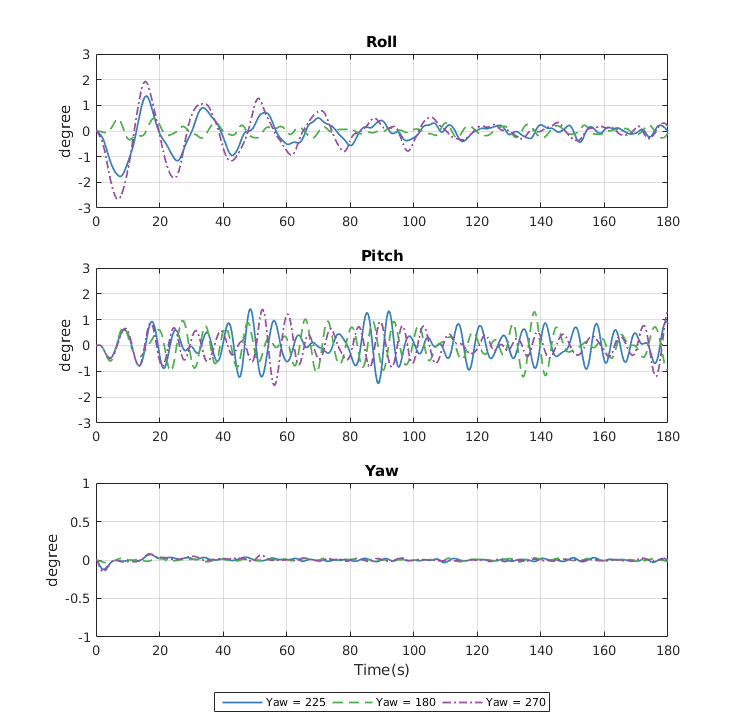
\includegraphics[width=0.7\textwidth]{figs/chp06/wave_30_height_25_comparision_rpy.pdf}	
	\caption{风向为$30\degree$,显著浪高为$2.5\ m$的海况下,三个坐标轴角速度的情况}
	\label{fig:wave_30_height_25_comparision_rpy}
\end{figure}

舰船由于受到风浪的干扰,横滚角和俯仰角都有一定的周期性震动,同理,可以得到舰船沉浮和三个转动角的频谱图,如图\ref{fig:wave_30_height_25_comparision_psw}所示。
 \begin{figure}[!ht]
	\centering
	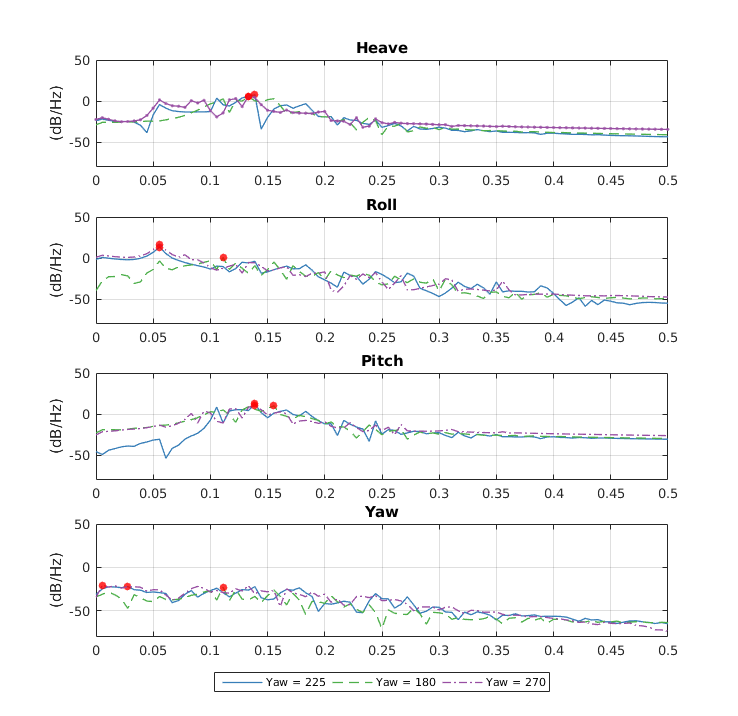
\includegraphics[width=0.7\textwidth]{figs/chp06/wave_30_height_25_comparision_psw.pdf}	
	\caption{风向为$30\degree$,显著浪高为$2.5\ m$的海况下,沉浮、横滚角、俯仰角和航向角的频谱图}
	\label{fig:wave_30_height_25_comparision_psw}
\end{figure}
其中红色标记为最大谱密度频率的峰值。最大偏差值如表\ref{lab:variance1}所示。可以看到,在逆风行驶的过程中,舰船沉浮赋值最小。
\begin{table}[]
	\centering
	\caption{船体受扰动后的各个参数的最大偏差}
	\label{lab:variance1}
	\begin{tabular}{cccc}
		\hline
		\textbf{船沉浮最大振幅(m)} & \textbf{\begin{tabular}[c]{@{}c@{}}舰船横滚角\\ 最大角度偏差($\degree$)\end{tabular}} & \textbf{\begin{tabular}[c]{@{}c@{}}舰船俯仰角\\ 最大角度偏差($\degree$)\end{tabular}} & \textbf{\begin{tabular}[c]{@{}c@{}}舰船航向角\\ 最大角度偏差($\degree$)\end{tabular}} \\ \hline
		0.49 & 1.35 & 1.46 & 0.08 \\
		0.79 & 0.41 & 1.04 & 0.04 \\
		0.84 & 2.66 & 1.54 & 0.07 \\ \hline
	\end{tabular}
\end{table}
最大功率谱密度频率如下表所示。通过表可以得到,舰船重心位置的扰动呈现明显的周期性,但最大功率谱中主频率相对较低,一般在$0.55\ Hz$到$0.2\ Hz$之间。

\subsection{期望着舰点运动分析}
通过海浪模型和舰船模型计算出船体重心位置俯仰、横滚、偏摆、沉浮、横荡和纵荡六个自由度扰动后,需要根据期望着舰点相对于船体重心的几何位置,进一步计算出期望着舰点位置受扰动的影响情况下相对于静止船体龙骨坐标系的坐标。
\begin{equation}
\begin{bmatrix}  x_{td} \\ y_{td} \\z_{td} \end{bmatrix} = \begin{bmatrix}	\cos \psi_{Sh} & \sin \psi_{Sh}  & 0     \\	 -\sin \psi_{Sh} & \cos \psi_{Sh}   & 0 \\ 	0   & 0 & 1 \end{bmatrix} \begin{bmatrix} \Delta x_{surge} \\ \Delta y_{sway} \\ \Delta z_{heave} \end{bmatrix} \\+ \mathcal{R}_{Sh,k}^{Sh,td}(\Delta \phi_{Sh}, \Delta \theta_{Sh}, \Delta \psi_{Sh}) \begin{bmatrix} \Delta x_{Sh,k}^{Sh,td} \\ \Delta y_{Sh,k}^{Sh,td} \\ \Delta z_{Sh,k}^{Sh,td} \end{bmatrix}
\end{equation}
由上式可以看到,期望着舰点位置的扰动主要受两部分影响,第一项主要描述舰船龙骨坐标系原点在沉浮、横荡和纵荡影响下的扰动量,第二项描述由于期望着舰点与龙骨坐标系原点存在固定偏移,俯仰、横滚和偏摆对期望期望着舰点位置的扰动量。
为计算期望着舰点运动扰动情况,设定期望着舰点的偏差为$x_{Sh,k}^{Sh,td} =50\ , y_{Sh,k}^{Sh,td}= 3\ ,z_{Sh,k}^{Sh,td}=7$。在舰船静止情况下,期望着舰点运动情况如下图所示。
 \begin{figure}[!ht]
	\centering
	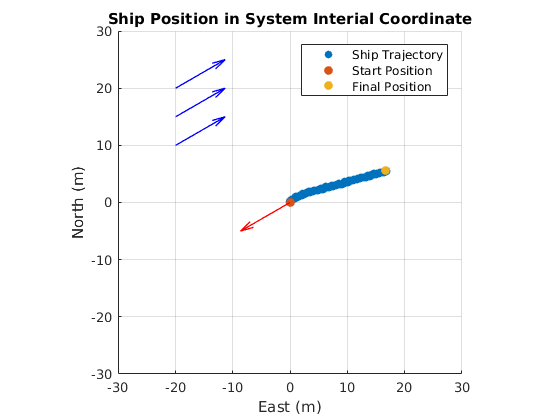
\includegraphics[width=0.7\textwidth]{figs/chp06/wave_30_height_25_yaw_30_speed_0_ship_motion.pdf}	
	\caption{舰船运动示意图}
	\label{fig:wave_30_height_25_yaw_30_speed_0_ship_motion}
\end{figure}
图中红色箭头为初始时舰船的朝向,在没有向前推力的情况下,舰船在海风的作用下向后侧运动。此时,期望着舰点变化情况如下图所示
 \begin{figure}[!ht]
	\centering
	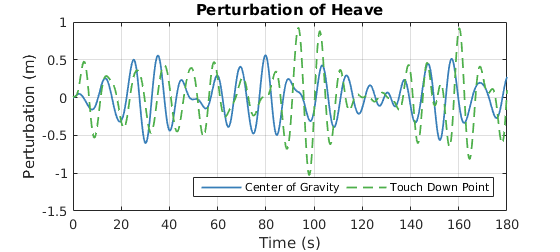
\includegraphics[width=0.7\textwidth]{figs/chp06/wave_30_height_25_yaw_30_speed_0_heave_compare.pdf}	
	\caption{期望着舰点频谱图}
	\label{fig:wave_30_height_25_yaw_30_speed_0_heave_compare}
\end{figure}

 \begin{figure}[!ht]
	\centering
	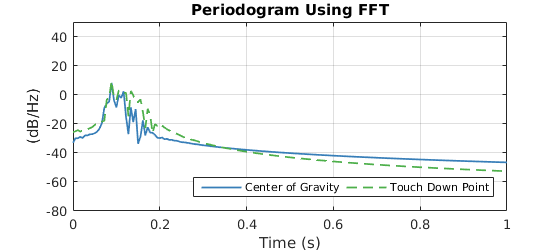
\includegraphics[width=0.7\textwidth]{figs/chp06/wave_30_height_25_yaw_30_speed_0_heave_psw_compare.pdf}	
	\caption{期望着舰点频谱图}
	\label{fig:wave_30_height_25_yaw_30_speed_0_heave_psw_compare}
\end{figure}
分析扰动图和谱密度图可以发现,在期望着舰点位置的沉浮赋值比舰船重心位置的要大,但二者的频域特性基本相同。

\section{无人机降落决策设计}
为简化无人机降落过程,本文把降落阶段划分为马歇尔点阶段、下降阶段和指令锁死阶段。其中从马歇尔阶段到下降阶段的过程中,地面引导系统可以捕获无人机,并进行跟踪和引导,在指令锁死阶段之前,无人机会经过决断窗口,判断是否复飞。如果无人机需要复飞,则需要经过复飞阶段和进近阶段后,飞行至光学系统捕获窗口附近。图\ref{fig:chp06_06_process}所示为该过程的示意图。
\begin{figure}[!tb]
	\centering
	\includegraphics[width=\textwidth]{figs/chp06/chp06_06_process.pdf}	
	\caption{无人机降落基本过程}
	\label{fig:chp06_06_process}
\end{figure}

一般而言,无人机的最终决断时间在接触甲板之前的1.5s至12.5s。定义下滑曲线的方位角误差为$\delta_h$,距离跑道中心线的误差为$\epsilon_h$,下滑曲线的俯仰角误差为$\delta_v$,距离期望下降曲线的高度差为$\epsilon_v$。无人机降落决策系统主要是通过上述多传感器的解算结果,在决断窗口根据无人机下降阶段的六个基本数据做出是否复飞的判断。这六个量分别为:
\begin{compactenum}
\item 跑道中心线的误差为$\epsilon_h$
\item 距离期望下降曲线的高度差为$\epsilon_v$
\item 无人机横滚角$\phi$
\item 无人机俯仰角$\theta$
\item 航母甲板下沉速率$\dot{h_c}$
\item 航母甲板侧滑速率$v_s$
\end{compactenum}

根据上述六个不同的基本数据指标,无人机主要面临一些六种危险如下表所示。
\begin{table}
	\centering
	\begin{tabular}{cccc}
		\hline
		\textbf{风险名称} & \textbf{符号表达} & \textbf{相关变量} & \textbf{状态描述}       \\ \hline
		撞击甲板下方 & PRS  & $e_v$ & 超过纵向最大负阈值  \\
		未接触拦阻索 & PUL  & $e_v$ & 超过纵向最大正阈值  \\
		横向偏差大  & POL  & 无   & 超过横向最大正负阈值 \\
		姿态偏差大  & PBA  & 无    & 着舰姿态偏差大    \\
		硬着舰    & PHL  & 无   & 超过沉降最大阈值   \\
		横向偏离跑道 & PRB  & 无    & 无          \\  \hline
	\end{tabular}
\end{table}
其中$P_{RS}$定义为
\begin{equation}
P_{RS}=\frac{1}{\sigma_v\sqrt{2\pi}}\int_{-\infty}^{e_{v,low}}\exp(-\frac{(x-\bar{e}_v)^2}{2\sigma_v^2})dx \\
=\frac{1}{2}(1+\text{erf}(\frac{e_{v, low}-\bar{e}_v}{\sigma_v\sqrt{2}}))
\end{equation}
其中误差函数定义为
\begin{equation}
\text{erf}(x)=\frac{2}{\sqrt{\pi}}\int_{0}^{x}e^{-t^2}dt
\end{equation}
假设六种情况发生的概率是相互独立的,由此定义无人机正常回收、复飞和失败的概率。上述误差量如图\ref{fig:chp06_05_landing_error}和图\ref{fig:chp06_06_landing_error_three_axis}所示。

\begin{align}
&P_{recover}=(1-P_{RS})(1-P_{UL})(1-P_{OL})(1-P_{BA})(1-P_{HL})(1-P_{RB}) \\
&P_{bolter}=(1-P_{RS})P_{UL}(1-P_{OL})(1-P_{BA})(1-P_{HL})(1-P_{RB}) \\
&P_{fail}=1-(1-P_{RS})(1-P_{OL})(1-P_{BA})(1-P_{HL})(1-P_{RB})
\end{align}




\begin{figure}[!tb]
	\centering
	\includegraphics[width=\textwidth]{figs/chp06/chp06_05_landing_error.pdf}	
	\caption{降落过程中的下滑轨迹误差}
	\label{fig:chp06_05_landing_error}
\end{figure}

\begin{figure}[!tb]
	\centering
	\includegraphics[width=\textwidth]{figs/chp06/chp06_06_landing_error_three_axis.pdf}	
	\caption{降落过程中的误差分布情况}
	\label{fig:chp06_06_landing_error_three_axis}
\end{figure}

\section{本章小结}
通过上述章节的分析可知,无人机在降落过程仅仅依靠可见光传感器进行引导降落存在一定风险。本章针对可见光传感器在远距离时,系统误差较大的情况,主要介绍了激光反射器、红外相机和超宽带雷达三种辅助传感器和EKF滤波器的设计,使得系统对无人机的识别和检测距离两个指标有所提高,对整体相对位置的解算精度进一步提升。此外,本文还使用经典方法对无人机的着舰点在海浪影响下的扰动情况在频域和时域进行分析,并设计无人机降落决策评价指标,使得引导系统的功能更加完备。
 
%\begin{algorithm2e}
%	\SetAlgoLined
%	\SetKwInOut{Input}{Input}
%	\SetKwInOut{Output}{Output}
%	\Input{Initialized sequence $\hat{\psi}(k),\ \ k=1,2,..., N$}
% 	
%	\KwResult{$x(k)$}
%	%initialization\;
%	\While{$\Sigma |x_{error}| \le \alpha$ and $|x^{*(i)} - x^{*(i-1)} | \le \beta$}
%	{
%		Update UAV states \;
%		$p(k+1) \leftarrow$ Update($p(k)$)\;
%		$\dot{p}(k+1) \leftarrow$ Update($\dot{p}(k)$)\;
%		${\phi}(k+1) \leftarrow$ Update(${\phi}(k)$)\;
%		Solve SCP using CVXGEN Solver\;
%		\For{$j\leftarrow 1$ \KwTo $N-1$}{
%			Calculate $x_{error}$ \;
%		}
%		Update $\hat{\psi}(k)^{i+1} = \hat{\psi}(k)^{i} $\;
%		Update Trust Region, $\rho(k)^{i+1} = \gamma_{path}(k)^{i} \rho(k)^{i}$ \;
%		$i = i + 1$
%	}
%	\caption{侧风扰动下的最优轨迹求解}
%\end{algorithm2e}
%
%\begin{algorithm2e}[H]
%	\SetAlgoLined
%	\KwData{this text}
%	\KwResult{how to write algorithm with \LaTeX2e }
%	initialization\;
%	\While{not at end of this document}{
%		read current\;
%		\eIf{understand}{
%			go to next section\;
%			current section becomes this one\;
%		}{
%			go back to the beginning of current section\;
%		}
%
%	}
%	\caption{How to write algorithms}
%\end{algorithm2e}
%
%\begin{algorithm2e}
%	\SetKwData{Left}{left}\SetKwData{This}{this}\SetKwData{Up}{up}
%	\SetKwFunction{Union}{Union}\SetKwFunction{FindCompress}{FindCompress}
%	\SetKwInOut{Input}{Input}\SetKwInOut{Output}{Output}
%	\Input{A bitmap $Im$ of size $w\times l$}
%	\Output{A partition of the bitmap}
%	\BlankLine
%	\emph{special treatment of the first line}\;
%	\For{$i\leftarrow 2$ \KwTo $l$}{
%		\emph{special treatment of the first element of line $i$}\;
%		\For{$j\leftarrow 2$ \KwTo $w$}{\label{forins}
%			\Left$\leftarrow$ \FindCompress{$Im[i,j-1]$}\;
%			\Up$\leftarrow$ \FindCompress{$Im[i-1,]$}\;
%			\This$\leftarrow$ \FindCompress{$Im[i,j]$}\;
%			\If(\tcp*[h]{O(\Left,\This)==1}){\Left compatible with \This}{\label{lt}
%				\lIf{\Left $<$ \This}{\Union{\Left,\This}}
%				\lElse{\Union{\This,\Left}}
%			}
%			\If(\tcp*[f]{O(\Up,\This)==1}){\Up compatible with \This}{\label{ut}
%				\lIf{\Up $<$ \This}{\Union{\Up,\This}}
%				\tcp{\This is put under \Up to keep tree as flat as possible}\label{cmt}
%				\lElse{\Union{\This,\Up}}\tcp*[h]{\This linked to \Up}\label{lelse}
%			}
%		}
%		\lForEach{element $e$ of the line $i$}{\FindCompress{p}}
%	}
%	\caption{disjoint decomposition}\label{algo_disjdecomp}
% 	\caption{使用SCP方法求解侧风扰动下的最优轨迹}
% \end{algorithm2e}
% 

